% Title: glps_renderer figure
% Creator: GL2PS 1.3.8, (C) 1999-2012 C. Geuzaine
% For: Octave
% CreationDate: Sat Apr 18 19:38:56 2015
\setlength{\unitlength}{1pt}
\begin{picture}(0,0)
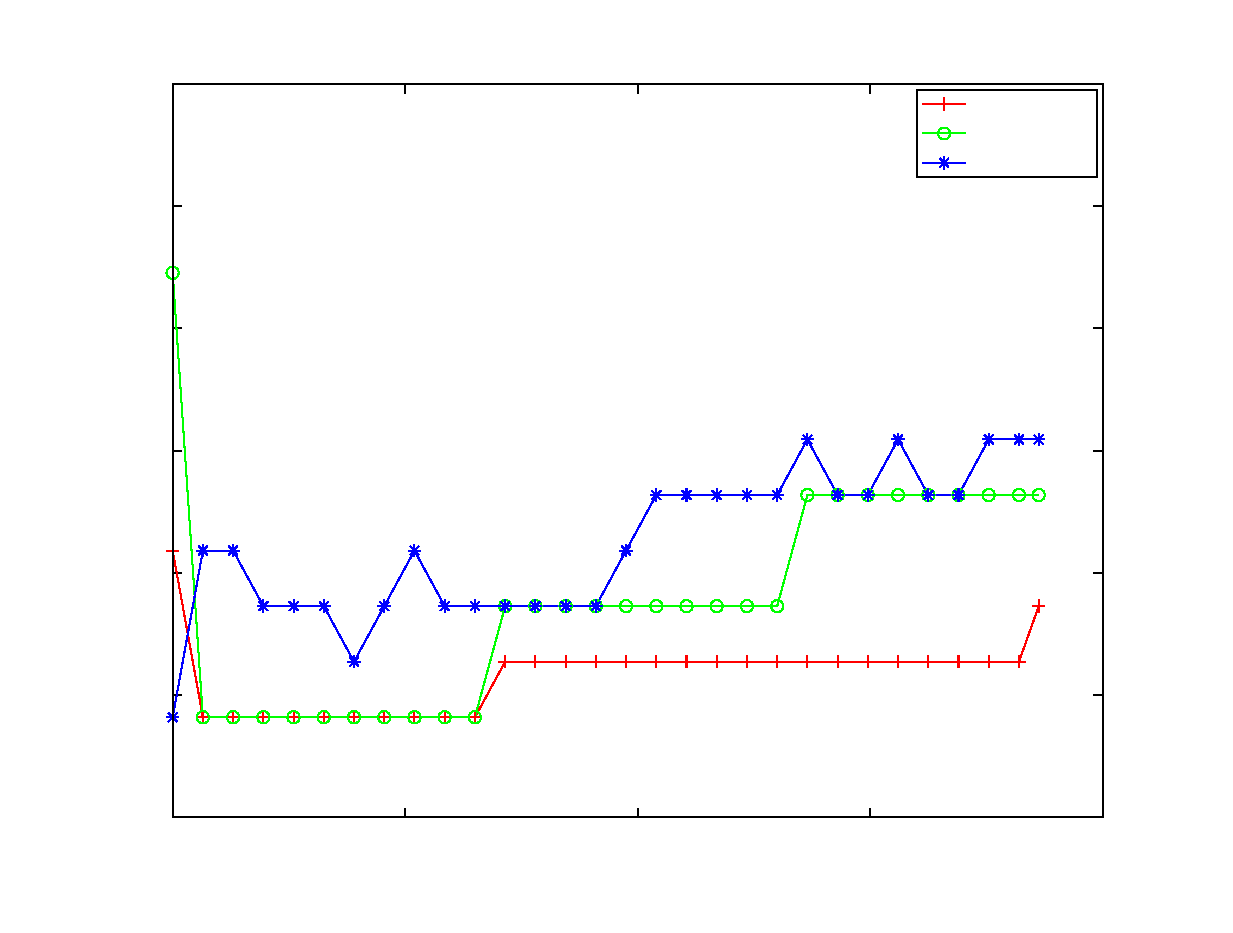
\includegraphics{sen-inc}
\end{picture}%
\begin{picture}(576,432)(0,0)
\fontsize{10}{0}
\selectfont\put(74.88,42.5189){\makebox(0,0)[t]{\textcolor[rgb]{0,0,0}{{0}}}}
\fontsize{10}{0}
\selectfont\put(186.48,42.5189){\makebox(0,0)[t]{\textcolor[rgb]{0,0,0}{{200}}}}
\fontsize{10}{0}
\selectfont\put(298.08,42.5189){\makebox(0,0)[t]{\textcolor[rgb]{0,0,0}{{400}}}}
\fontsize{10}{0}
\selectfont\put(409.68,42.5189){\makebox(0,0)[t]{\textcolor[rgb]{0,0,0}{{600}}}}
\fontsize{10}{0}
\selectfont\put(521.28,42.5189){\makebox(0,0)[t]{\textcolor[rgb]{0,0,0}{{800}}}}
\fontsize{10}{0}
\selectfont\put(69.8755,47.52){\makebox(0,0)[r]{\textcolor[rgb]{0,0,0}{{0.1}}}}
\fontsize{10}{0}
\selectfont\put(69.8755,106.2){\makebox(0,0)[r]{\textcolor[rgb]{0,0,0}{{0.2}}}}
\fontsize{10}{0}
\selectfont\put(69.8755,164.88){\makebox(0,0)[r]{\textcolor[rgb]{0,0,0}{{0.3}}}}
\fontsize{10}{0}
\selectfont\put(69.8755,223.56){\makebox(0,0)[r]{\textcolor[rgb]{0,0,0}{{0.4}}}}
\fontsize{10}{0}
\selectfont\put(69.8755,282.24){\makebox(0,0)[r]{\textcolor[rgb]{0,0,0}{{0.5}}}}
\fontsize{10}{0}
\selectfont\put(69.8755,340.92){\makebox(0,0)[r]{\textcolor[rgb]{0,0,0}{{0.6}}}}
\fontsize{10}{0}
\selectfont\put(69.8755,399.6){\makebox(0,0)[r]{\textcolor[rgb]{0,0,0}{{0.7}}}}
\fontsize{10}{0}
\selectfont\put(298.08,31.5188){\makebox(0,0)[t]{\textcolor[rgb]{0,0,0}{{it}}}}
\fontsize{10}{0}
\selectfont\put(50.8755,223.56){\rotatebox{90}{\makebox(0,0)[b]{\textcolor[rgb]{0,0,0}{{sen}}}}}
\fontsize{10}{0}
\selectfont\put(458.195,389.829){\makebox(0,0)[l]{\textcolor[rgb]{0,0,0}{{Kendalls}}}}
\fontsize{10}{0}
\selectfont\put(458.195,375.772){\makebox(0,0)[l]{\textcolor[rgb]{0,0,0}{{Spearmans}}}}
\fontsize{10}{0}
\selectfont\put(458.195,361.715){\makebox(0,0)[l]{\textcolor[rgb]{0,0,0}{{Pearsons}}}}
\end{picture}
